\section {Evaluation}
\label{sec:eval}

We evaluated SpotWeb with eight widely used open source frameworks,
which differ in size and purpose. In our evaluation, we investigate the
following research questions. (1) What is the percentage of hotspot and coldspot 
classes and methods among the total number of classes and methods in each framework, respectively? 
This research question helps to characterize the usages of a framework and reuse
efforts of the framework. (2) Is the subset of classes and methods detected
as hotspots indeed useful in helping effective framework reuse? We address the preceding question by 
showing that detected hotspots include classes and methods of a framework reused by a real application.
This evaluation helps to show that our approach can help reduce the efforts
of users by suggesting a subset of classes and methods as hotspots.
(3) What is the effectiveness of our hotspot detection in terms of precision and
recall? We address the preceding question through two evaluations. First, we compare
the detected hotspot classes with the classes described in the documentation associated
with the frameworks. Second, we compare the detected hotspot classes with 
the hotspots detected by a previous related approach by Viljamaa~\cite{viljamaa:reverse}.

The subjects used in our evaluation and their
characteristics such as the number of classes and methods are shown
in Columns ``Classes'' and ``Methods'' of Table~\ref{tab:subjects}.
Column ``Samples'' of Table~\ref{tab:subjects} shows the number of
code examples gathered from Google code search~\cite{GCSE} and Column ``KLOC'' shows the total number of
kilo lines of Java code analyzed by SpotWeb for identifying hotspots
and coldspots. One of the major advantages of SpotWeb compared to
other approaches is the large number of analyzed code examples
that can help detect hotspots and coldspots effectively.

\setlength{\tabcolsep}{1pt}
\begin{table*}[t]
\begin{CodeOut}
\begin{center}
\begin {tabular} {|l|c|c|c|c|l|}
\hline
Subject&\# Classes&\# Methods&\# Samples&\# KLOC&\CenterCell{URL}\\
\hline Log4j&207&1543&9768&2064&logging.apache.org/log4j\\
\hline JUnit&56&531&8891&1558&www.junit.org\\
\hline JGraphT&177&931&289&30&jgrapht.sourceforge.net\\
\hline Grappa&44&561&2071&1978&www.graphviz.org\\
\hline OpenJGraph&210&1365&1076&113&openjgraph.sourceforge.net\\
\hline JUNG&461&3241&2390&353&jung.sourceforge.net\\
\hline BCEL&357&3048&5225&1219&jakarta.apache.org/bcel\\
\hline Javassit&249&2149&3226&631&www.csg.is.titech.ac.jp/chiba/javassist\\
\hline
\end{tabular}
\centering \caption {\label{tab:subjects} Subjects used for evaluating SpotWeb.}
\end{center}
\end{CodeOut}
\end{table*}
\Comment{%---------------------------------------------------------------------------------------------
\subsection{Subjects}
\label{sec:subjects}
Log4j is a library used for inserting
logs in source code. JUnit is the
\emph{de facto} standard unit testing framework for the Java
programming language. JGraphT, Grappa, OpenJGraph, and JUNG are four
graph libraries that provide several graph manipulation utilities.
BCEL and Javassit are libraries that provide functionality for
creating, analyzing, and manipulating Java class files.
}

\setlength{\tabcolsep}{1pt}
\begin{table*}[t]
\begin{CodeOut}
\begin{center}
\begin {tabular} {|l|c|c|c|c|c|c|c|c|c|c|c|}
\hline
Subject&\# Classes&\multicolumn{5}{|c|}{Hotspot classes}&\multicolumn{2}{|c|}{Coldspot classes}&\multicolumn{3}{|c|}{Hotspot methods}\\
\cline{3-12}
&&\# Classes&\%&\# Templ&\# Hooks&\# Depend&\#Classes&\%&\# Total Methods&\# Hotspot Methods&\%\\
\hline Log4j        &207&56&27.05&35&11&22&131&63.28&1543&299&19.38\\
\hline JUnit            &56&14&25&8&3&7&22&39.28&531&77&14.50\\
\hline JGraphT      &177&41&23.16&20&8&0&135&76.27&931&102&10.96\\
\hline Grappa           &44&16&36.36&11&2&3&23&52.27&561&50&8.91\\
\hline OpenJGraph   &210&35&16.67&21&6&7&172&81.90&1365&76&5.57\\
\hline JUNG             &461&195&42.29&128&17&109&222&48.15&3241&569&17.55\\
\hline BCEL             &357&121&33.89&74&9&59&192&53.78&3048&580&19.03\\
\hline Javassit     &249&70&28.11&57&4&14&175&70.28&2149&371&17.26\\
\hline
\end{tabular}
\centering \caption {\label{tab:hotanddead} Evaluation results showing the
detected hotspots and coldspots.}
\end{center}
\end{CodeOut}
\end{table*}
%---------------------------------------------------------------------------------------------
\subsection{Statistics of Hotspots and Coldspots}
\label{sec:hotspotsres}
We next address the first question on the percentage of classes and methods classified
as hotspots or coldspots. These statistics help identify the possibilities of reuse in a framework
and the amount of efforts required by a new user in getting familiar with the given framework.
Table~\ref{tab:hotanddead} shows the statistics of hotspots in all frameworks.
Column ``Subject'' shows the name of the input framework. Columns ``Hotspot classes''
and ``Coldspot classes'' present the number of classes classified as hotspots and
coldspots, respectively. Column ``Hotspot methods'' shows the number of methods identified
as hotspot methods. Sub-columns ``Classes'' and ``\%'' of Column ``Hotspot classes'' show the number of hotspot classes
and their percentages among the total number of classes. Columns ``Templ'', ``Hooks'', and ``Depend''
give the number of template hierarchies, hook hierarchies, and their dependencies, respectively. Sub-columns
``Classes'' and ``\%'' of Column ``Coldspots'' show the number of coldspot classes and their percentages.

\begin{figure}[t]
\centering
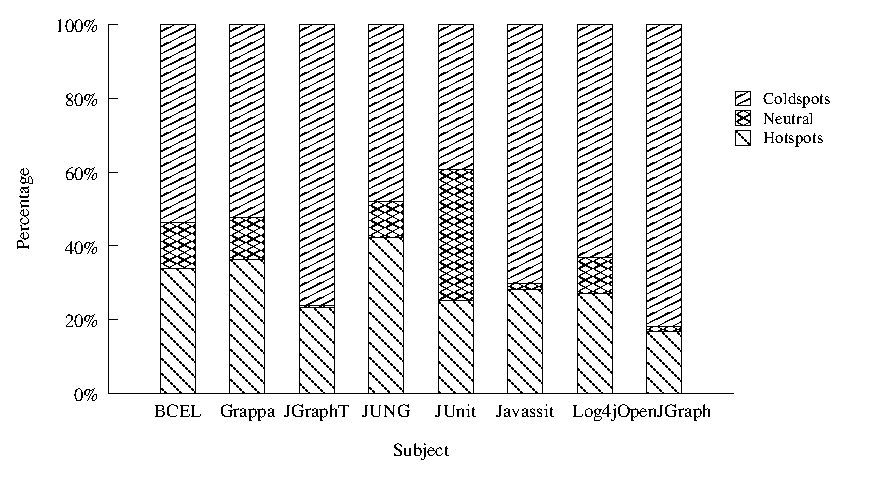
\includegraphics[scale=0.65,clip]{figs/hotanddeadstats.eps}
\caption{\label{fig:hotdeadstats} Distribution of hotspot and coldspot percentages in all subject frameworks.} 
\end{figure}

Our results show that the percentage of hotspots for all subjects
ranges from 16\% to 42\%, whereas the percentage of coldspots ranges
from 39\% to 82\%. These statistics help identify the efforts in reusing 
a given framework. For example, the required efforts for reusing 
the JUnit framework can be low compared to the efforts required for reusing
the JUNG library \Fix{because the number of hotspots of the JUNG library is
greater than the number of hotspots of the JUnit framework.}
Figure~\ref{fig:hotdeadstats} presents the
distribution of hotspot and coldspot percentages of all subjects. 
The distribution chart shows that OpenJGraph and JGraphT frameworks
have the lowest percentage of hotspots and the highest percentage of
coldspots. This scenario can provide a hint that only a few classes of these
frameworks are often reused. In the figure, we also show a new classification called
``Neutral'', which represents classes that do not belong to either
the hotspot or coldspot category. The graph shows that the
percentage of classes in the Neutral category is relatively low for
all subjects except JUnit. This characteristic indicates that a class
is either reused heavily or is never reused, and only in a few cases
a class is occasionally reused.

We next describe a few example hotspot classes detected for the four graph libraries
JGraphT, Grappa, OpenJGraph, and Grappa. Each graph library provides several
different types of graphs. For example, the JUNG library provides 
graphs such as \CodeIn{DirectedGraph}, \CodeIn{ArchetypeGraph},
and \CodeIn{HyperGraph}.  SpotWeb identified the graph type that is commonly
used among all different types provided by each library. For example, SpotWeb
identified that graphs \CodeIn{DefaultListenableGraph}, \CodeIn{DirectedSparseGraph}, \CodeIn{DirectedGraphImpl},
and \CodeIn{Graph} are the commonly used graph types in JGraphT, JUNG, OpenJGraph, and Grappa
graph libraries, respectively. 
%----------------------------------------------------------------------------------------------
\subsection{Utilities of Hotspots}
\label{sec:hotspotuse}
We next try to address the second question on whether the subset of classes and methods
detected as hotspots is indeed useful in helping effective framework reuse. 
We use DNSJava\footnote{\url{http://www.dnsjava.org/}},
a popular framework that provides implementation of DNS in Java, as an input framework. 
We choose DNSJava for two primary reasons: DNSJava is used as a subject in several
previous approaches and the DNSJava webpage provides example applications that can be used to validate
the detected hotspots. We classify all DNSJava reusing applications available on the web through Google code search
(except the James\footnote{\url{http://james.apache.org/}} 
application) as training applications for SpotWeb to detect 
hotspots of DNSJava. We validate the detected hotspots using James as a test application.
We selected James as the test application, because James is one of the example applications
described in the webpage of DNSJava.

To show the utility of the detected hotspots, we identify the DNSJava classes 
and methods that are reused by James and compute the percentage of those classes detected
by SpotWeb. Table~\ref{tab:jamesres} shows the results of our evaluation.
DNSJava includes 151 classes and 1224 methods. \Comment{SpotWeb identified 50 classes and 244 methods
as hotspot classes and methods, respectively.} The
James application reused 17 classes and 18 methods of DNSJava. James also used 1 exception
class and 7 constants declared by DNSJava. Table~\ref{tab:jamesres} shows
the evaluation results. Columns ``James'' and ``SpotWeb'' show the 
classes, methods, exceptions, and constants used by James and are among
the detected hotspots by SpotWeb. The hotspots detected by SpotWeb
include 16 classes and 16 methods reused by James. Moreover, SpotWeb also correctly
detected all seven constants referred by James. SpotWeb could not detect one hotspot
class, called \CodeIn{Resolver}. The primary reason is that \CodeIn{Resolver} is an interface
and gathered code examples do not include any usages of the \CodeIn{Resolver} interface.
This evaluation shows that the detected hotspots are indeed useful in helping
effective framework reuse and can help reducing the efforts of a programmer unfamiliar
to the framework by suggesting a subset of classes and methods as hotspots.

\setlength{\tabcolsep}{1pt}
\begin{table}[t]
\begin{CodeOut}
\begin{center}
\begin {tabular} {|l|c|c|c|}
\hline
&James&SpotWeb&\%\\
\hline Classes&17&16&94.11\\
\hline Methods&18&16&88.88\\
\hline Exceptions&1&1&100\\
\hline Constants&7&7&100\\
\hline
\end{tabular}
\centering \caption {\label{tab:jamesres} Hotspots of DNSJava reused by James.}
\end{center}
\end{CodeOut}
\end{table}


%---------------------------------------------------------------------------------------------
\subsection{Effectiveness of Hotspot Detection}
We next address the third question regarding the effectiveness of our hotspot detection
with respect to precision and recall through two evaluations. First, we compare
the detected hotspots of JUnit and Log4j frameworks with available documentations.
Second, we compare SpotWeb results with the results of a previous approach 
by Vijamaa~\cite{viljamaa:reverse}.

%---------------------------------------------------------------------------------------------
\subsubsection{Comparison with documentation}
We next analyze the effectiveness of hotspot detection through the
evaluation results with Log4j and JUnit frameworks. The primary
reason for selecting Log4j\footnote{\url{http://logging.apache.org/log4j/docs/manual.html}}
and JUnit\footnote{\url{http://junit.sourceforge.net/doc/cookstour/cookstour.htm}}
for analysis is the availability of their documentation that can
help validate the detected hotspots. 

Log4j provides several features such as Appenders and Layouts, and
for each such feature Log4j provides several classes. For example, Log4j
provides classes \CodeIn{ConsoleAppender} and \CodeIn{JDBCAppender} for the appender feature.
Among those several classes provided for each feature, a few classes are
much more often used than other classes. The features described in the documentation of Log4j are shown in
Columns ``Feature'' and ``Description'' of Table~\ref{tab:hdresults}. Column
``Class'' shows the commonly used classes for each feature. Each of these
classes serves as starting points for using those features.

\setlength{\tabcolsep}{1pt}
\begin{table*}[t]
\begin{CodeOut}
\begin{center}
\begin {tabular} {|l|l|l|c|c|}
\hline
Feature&\CenterCell{Description}&\CenterCell{Class}&Rank&Type\\
\hline Loggers&Log the messages of several levels&Category&1&\CodeIn{TEMPLATE}\\
\hline &&Logger&9&\CodeIn{HOOK}\\
\hline &&Level&4&\CodeIn{HOOK}\\
\hline Appenders&Allows logging to multiple destinations&ConsoleAppender&11&\CodeIn{TEMPLATE}\\
\hline &&FileAppender&16&\CodeIn{TEMPLATE}\\
\hline Layouts&Helps to format the logging request&PatternLayout&5&\CodeIn{TEMPLATE}\\
\hline &&SimpleLayout&13&\CodeIn{TEMPLATE}\\
\hline Configurators&Helps to configure Log4j&BasicConfigurator&2&\CodeIn{TEMPLATE}\\
\hline &&PropertyConfigurator&3&\CodeIn{TEMPLATE}\\
\hline &&DOMConfigurator&7&\CodeIn{TEMPLATE}\\
\hline Loaders&Helps to load resources&Loader&27&\CodeIn{TEMPLATE}\\
\hline NDC&Nested diagnostic constant&NDC&12&\CodeIn{TEMPLATE}\\
\hline
\end{tabular}
\centering \caption {\label{tab:hdresults} Hotspots described in the Log4j documentation.}
\end{center}
\end{CodeOut}
\end{table*}

SpotWeb identified 56 classes as hotspots in Log4j for
the $HT$ percentage of 15\%, and these classes captured 
all 12 starting points described in the
documentation resulting in a recall of 100\%. In constrast, the
precision is 21.42\%.  Column ``Rank'' of Table~\ref{tab:hdresults} presents the rank 
of each documented class among the total number of 
hotspots detected by SpotWeb. Column ``Type'' shows
whether the detected hotspot is a \CodeIn{TEMPLATE} or a
\CodeIn{HOOK}. The table also shows that except the
\CodeIn{Loader} class, all other 11 hotspot classes are ranked among
the top 16 classes of the total 56 classes. Therefore, a user who
plans to reuse classes of Log4j can refer to the first 16
classes suggested by SpotWeb to identify where to start reusing the
framework.

We used the cookbook provided with the JUnit framework to verify the
detected hotspots. Hotspots detected in the JUnit framework are
shown in Figure~\ref{fig:hotspotexample}. SpotWeb identified 
5 out of 6 hotspot classes described in the cookbook resulting in a recall of
83.33\% and precision 35.71\%. 

\begin{figure*}[t]
\centering
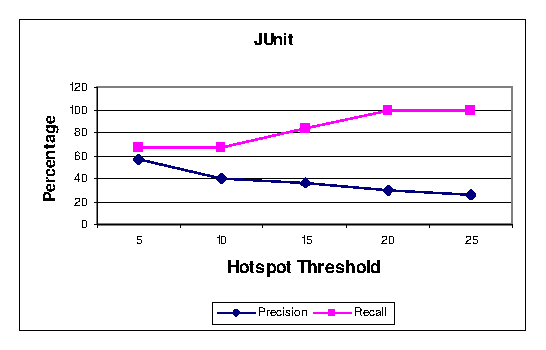
\includegraphics[scale=0.68,clip]{figs/junit.eps}
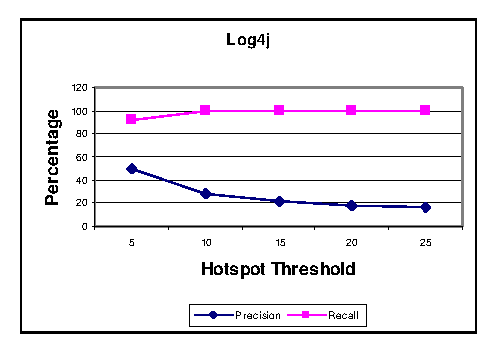
\includegraphics[scale=0.68,clip]{figs/log4j.eps}
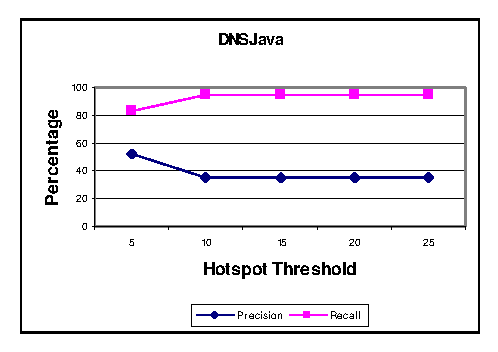
\includegraphics[scale=0.68,clip]{figs/dnsjava.eps}
\caption{\label{fig:precrecall}Precision and Recall for five $HT$ values with JUnit, Log4j, and DNSJava} 
\end{figure*}

We next describe our empirical analysis with several $HT$ values and describe
why we use $HT$ of 15\% to identify hotspots. Figure~\ref{fig:precrecall}
shows the results with three subjects and several threshold values ranging from 5\% to 25\%.
With the increase in the threshold value, the precision decreases
and the recall increases. \Fix{Although decrease in the precision is common with 
increase in the threshold value, the figure shows that the precision
decreases rapidly with increase in the threshold value. This phenomenon
shows that the real hotspots of these frameworks are beyond those hotspots
calculated based on the documentation because the documentation
of existing frameworks is often outdated. This evaluation shows the necessity
of an approach such as SpotWeb that can automatically infer hotspots
from the applications that are already reusing the API classes and methods of the input framework.}

In our implementation, we used $HT$ as 15\%
as this threshold value has high recall with reasonable precision.
The primary reason for inclining toward a high recall with low precision
is that the framework users do not miss any hotspot classes. Furthermore,
our ranking mechanism helps to give higher priority to those
hotspot classes that are described in the documentation compared
to the other classes as shown in Table~\ref{tab:hdresults}.
%---------------------------------------------------------------------------
\subsubsection{Comparison with Viljamaa's approach}
We next compare the results of SpotWeb with the results of a previous related approach by Viljamaa~\cite{viljamaa:reverse}
for the JUnit framework. Their approach also recovers the hotspots of a framework
by using the source code of the framework and a set of available example applications. Their approach
uses concept analysis~\cite{ganter:concept} for recovering hotspots of the framework. As both approaches target
a similar problem, we compared the results of SpotWeb for the JUnit framework with the
results of their approach. Viljamaa's approach detected a total of 7 classes. 
SpotWeb detected 5 classes among these 7 classes. The 2 missing classes
are \CodeIn{ExceptionTestCase} and \CodeIn{ActiveTestSuite}. However, both
these classes are not described in the available documentation of JUnit.
SpotWeb is not able to detect these classes because of low 
support among gathered code examples. SpotWeb detected 4 new classes and several
new methods that are not detected by Viljamaa's approach and are described in the documentation. 
For example, classes of JUnit such as \CodeIn{Assert}, \CodeIn{TestResult},
and \CodeIn{TestFailure} (shown in Figure~\ref{fig:hotspotexample}) 
are often used and only detected by SpotWeb. Similarly, for the
\CodeIn{Testcase} class, the \CodeIn{tearDown} method is also often used along with
the \CodeIn{setUp} method. Viljamaa's approach detected only the \CodeIn{setUp} method, whereas
SpotWeb detected both \CodeIn{setUp} and \CodeIn{tearDown} methods as hotspot methods.
These results show that SpotWeb can perform better than Viljamaa's approach.
Furthermore, Viljamaa's approach requires the users to have 
some initial knowledge of the structure and hotspots of the input framework that is being analyzed.
In contrast, our approach does not require the users to have any knowledge regarding the 
input framework.

\Comment{
%---------------------------------------------------------------------------------------------
\subsection{Coldspots}
\label{sec:coldspotsres}
The coldspot classes identified by SpotWeb in each framework are
shown in Column ``Coldspots'' in Table~\ref{tab:hotanddead}. The sub-columns
``Classes'' and ``\%'' show the number of coldspot classes and the percentage
among the total number of classes. SpotWeb detected several coldspot classes in each subject
framework. In general, coldspot classes help users explore
alternate commonly used classes as they are more exercised and may have lower chance
of having bugs. For example, a user of the Log4j library wants to use the layout feature
that is provided with several classes such as \CodeIn{DateLayout} and \CodeIn{PatternLayout}.
As \CodeIn{DateLayout} is detected as a coldspot, SpotWeb
recommends to use other classes such as \CodeIn{PatternLayout}. }

